\documentclass[a4paper]{article}

\usepackage{graphicx}
\usepackage{amsmath,amssymb}
\usepackage{minted}
\usepackage{multirow}
\usepackage{float}
\usepackage{todonotes}
\usepackage{forest}
\usepackage{xstring}
\usepackage{xcolor}
\usepackage[most]{tcolorbox}
\usepackage{xparse}
\usepackage{natbib}

\usetikzlibrary{graphs,graphdrawing}
\usegdlibrary{layered}

% for external graphviz
\input{/home/donkarlo/Dropbox/repo/nd_ai_project/src/nd_ai/knoweldge_representation/language/formal/computer/programming/tex/latex/code_clips/external_graphviz.tex}

% for tags
\input{/home/donkarlo/Dropbox/repo/nd_ai_project/src/nd_ai/knoweldge_representation/language/formal/computer/programming/tex/latex/parts/control_sequence/kind/semtag/semtag.tex}

% for links
\input{/home/donkarlo/Dropbox/repo/nd_ai_project/src/nd_ai/knoweldge_representation/language/formal/computer/programming/tex/latex/code_clips/seehere.tex}

\title{Street-Level and 360-Degree Imagery}
\date{}
\author{Mohammad Rahmani}

\begin{document}
    \maketitle
    
    
    \section{Street-Level and 360-Degree Imagery}
        Street-level and $360^\circ$ imagery captures buildings from the viewpoint of a pedestrian, bicycle, or vehicle.
        It can provide evidence about facade materials, roof edges, gutters, visible roof coverings, dormers, damage, and features hidden in top-down imagery.
        Geotagged image sequences can also help verify building identity and resolve uncertainty when aerial sources are outdated or obstructed.
        Its weaknesses are incomplete coverage, privacy filtering, inconsistent capture dates, severe occlusion, and limited visibility of roofs on tall or narrow streets.
        Open street imagery can be explored through Mapillary \seeherefooter{https://www.mapillary.com/} and the Mapillary web application \seeherefooter{https://www.mapillary.com/app/}.
        
        \begin{figure}[H]
            \centering
            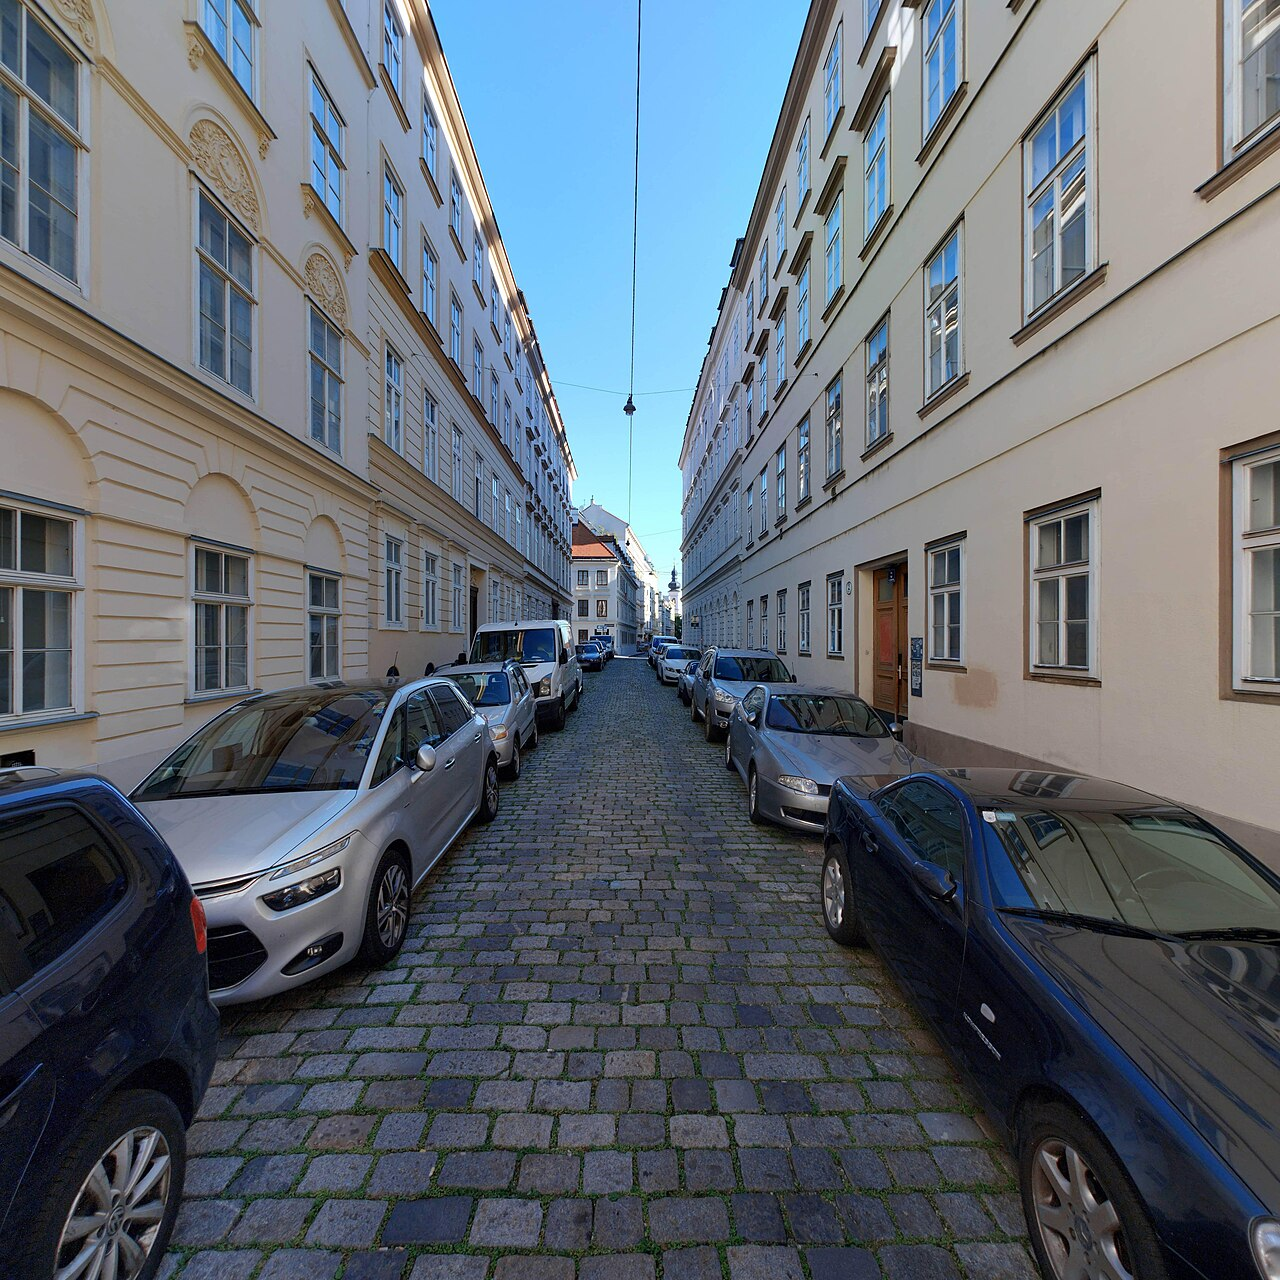
\includegraphics[width=0.74\textwidth]{images/street_level_360_imagery_example.jpg}
            \caption{Street-level Mapillary image from Schlösselgasse in Vienna.}
        \end{figure}
        \noindent\small Image source, author, and licence information: \seeherefooter{https://commons.wikimedia.org/w/index.php?oldid=1191706066}.\normalsize
        
%        \bibliographystyle{plainnat}
%        \bibliography{/home/donkarlo/Dropbox/repo/nd_shared_research/bibliography/bibliography.bib}
\end{document}
